\documentclass{article}

\usepackage{graphicx}
\usepackage{tikz}
\usepackage{tikzsymbols}
\usetikzlibrary{calc,patterns,shapes.geometric}
\pagestyle{empty}
\usepackage[margin=0pt]{geometry}
\geometry{papersize={14in,12in}}

\def\centerarc[#1](#2)(#3:#4:#5){\draw[#1] ($(#2)+({#5*cos(#3)},{#5*sin(#3)})$) arc (#3:#4:#5);}

\begin{document}
	\begin{figure}
		\centering
		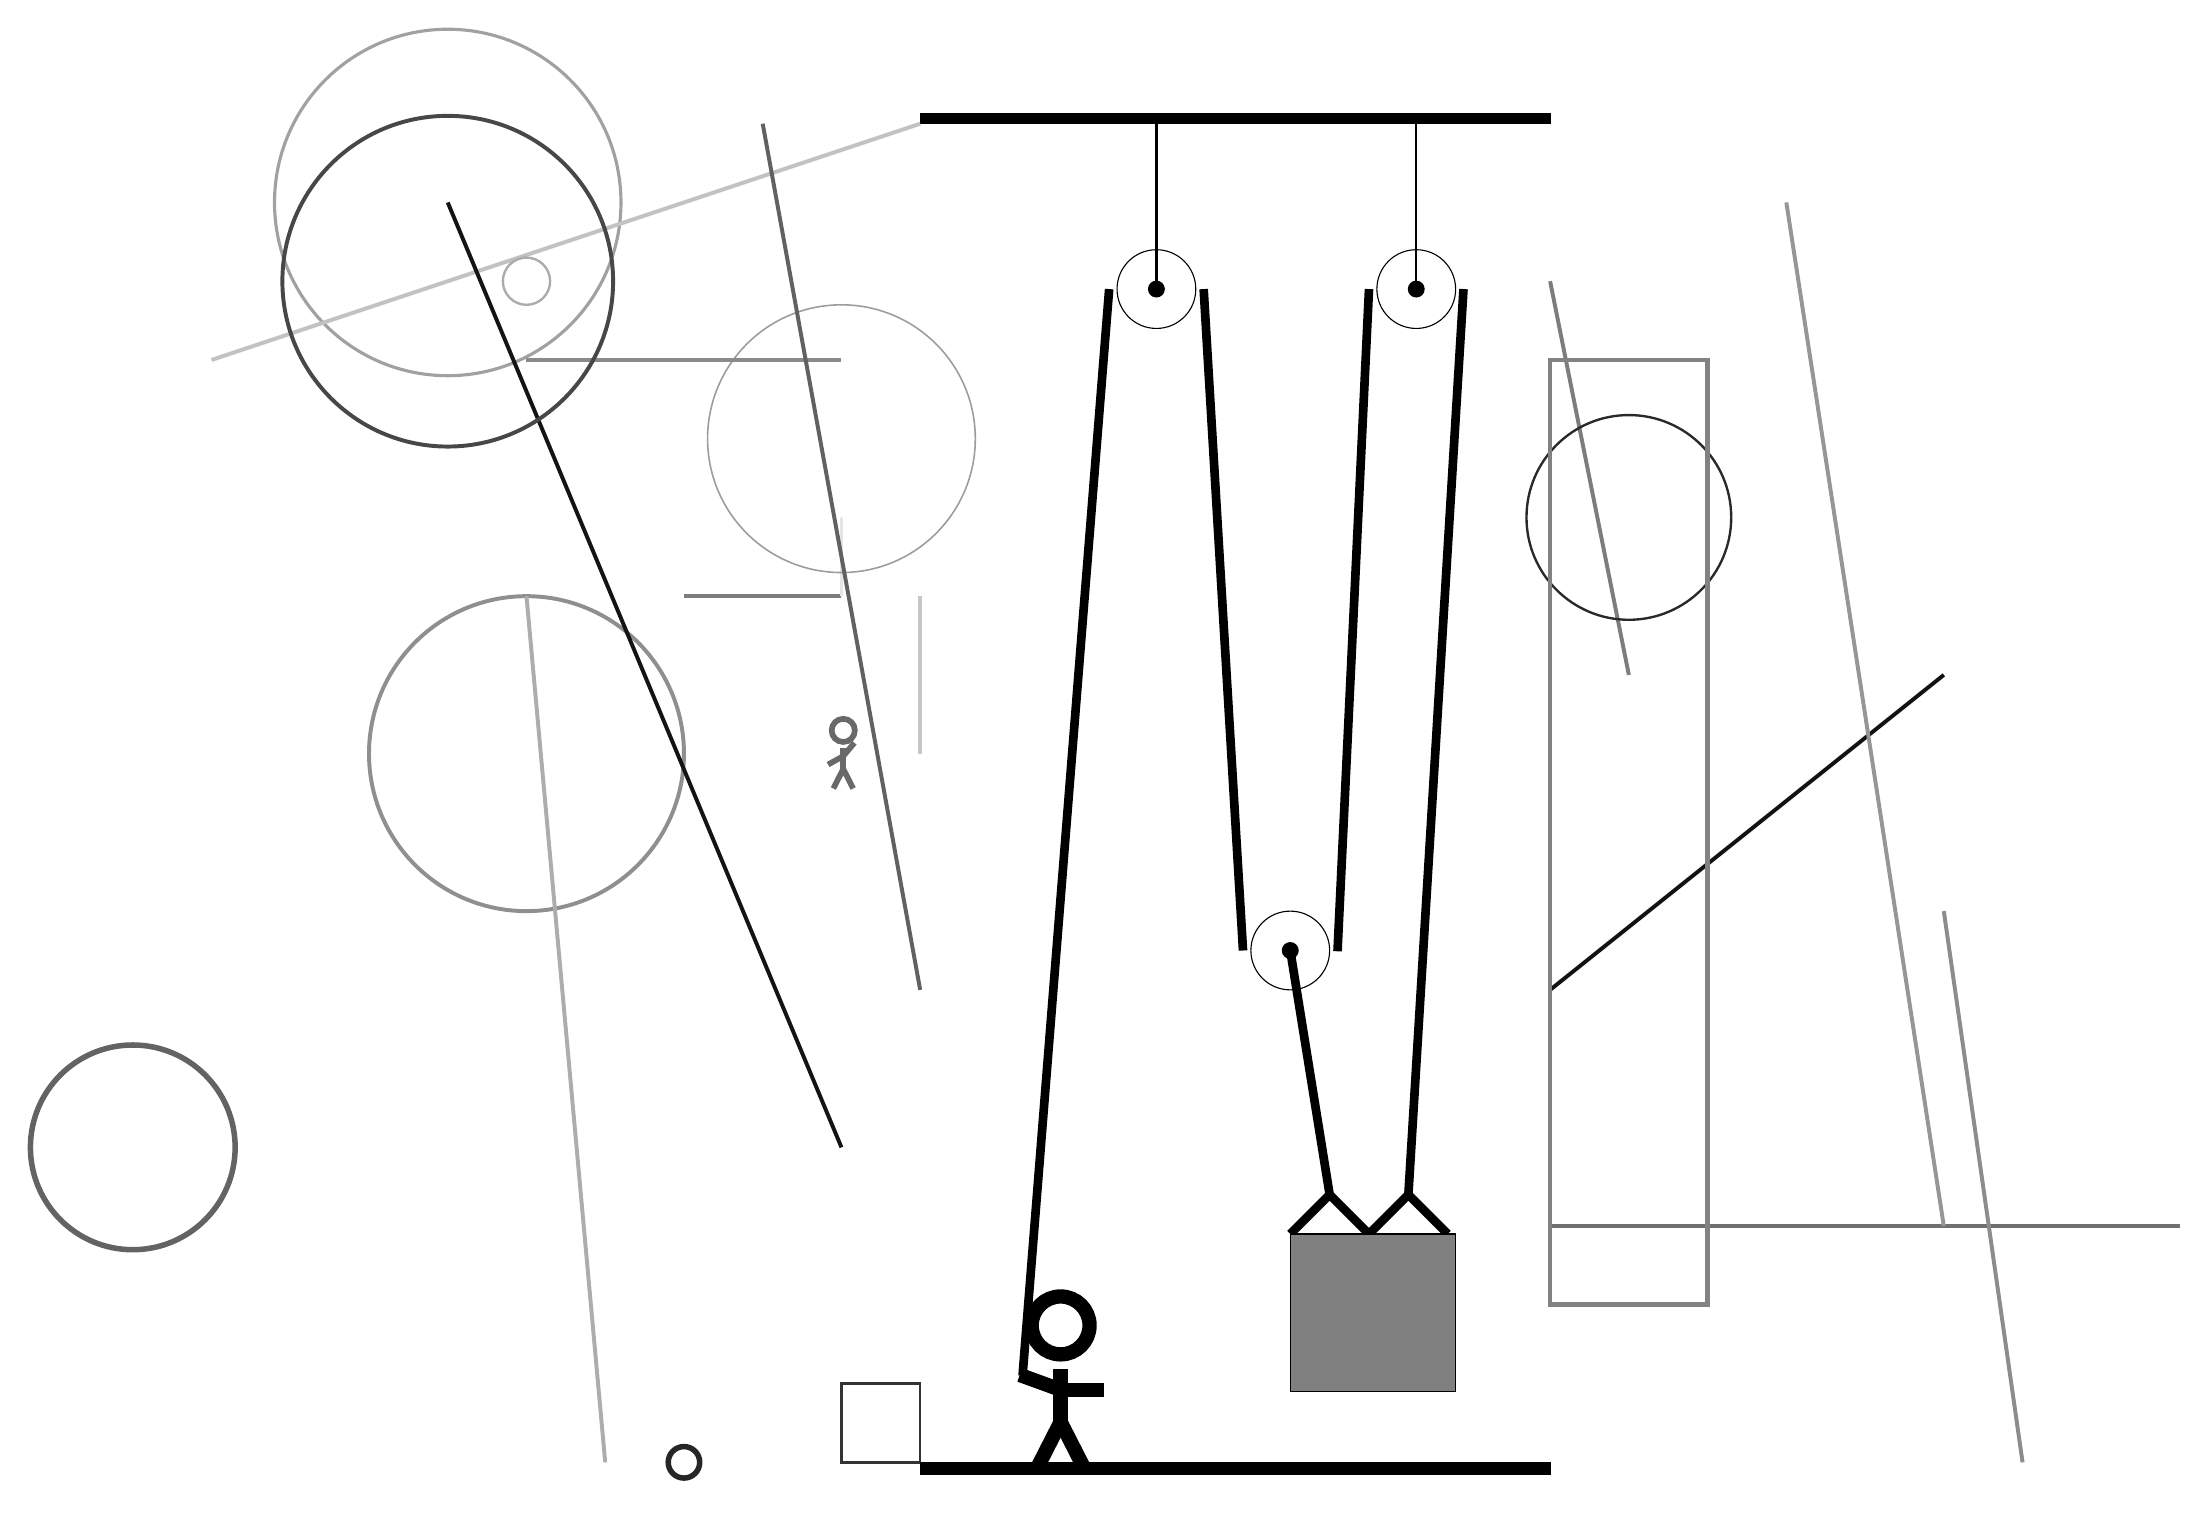
\begin{tikzpicture}
			%%%%% START %%%%%
			
			\draw[fill=black] (-2, 14) rectangle (6, 14.125);
			
			\draw (1, 11.9) circle (0.5);
			\draw[fill=black] (1, 11.9) circle (0.1);
			\draw[thick] (1, 11.9) -- (1, 14);
			
			\draw (4.3, 11.9) circle (0.5);
			\draw[fill=black] (4.3, 11.9) circle (0.1);
			\draw[thick] (4.3, 11.9) -- (4.3, 14);
			
			\draw (2.7, 3.5) circle (0.5);
			\draw[fill=black] (2.7, 3.5) circle (0.1);
			
			\draw[line width=0.5mm, color=black!56](6, 0) -- (14, 0);
			
			\draw [line width=0.4mm, color=black!37](-8, 13) circle (2.2);
			\draw [line width=0.7mm, color=black!61](-12, 1) circle (1.3);
			\node[line width=0.2mm, color=black!59] at (-3, 6) {\Strichmaxerl[4][29][50]};
			\draw[line width=0.5mm, color=black!45](11, 4) -- (12, -3);
			\draw [line width=0.5mm, color=black!44](-7, 6) circle (2.0);
			\draw[line width=0.5mm, color=black!51](-3, 8) -- (-5, 8);
			\draw[line width=0.5mm, color=black!93](6, 3) -- (11, 7);
			\draw[line width=0.3mm, color=black!80] (-2, -2) rectangle (-3, -3);
			
			\draw[line width=0.3mm, color=black!10] (-3, 8) rectangle (-3, 9);
			
			\draw[line width=0.5mm, color=black!51](6, 12) -- (7, 7);
			
			\draw[line width=0.5mm, color=black!24](-2, 14) -- (-11, 11);
			\draw [line width=0.2mm, color=black!39](-3, 10) circle (1.7);
			
			\draw[line width=0.5mm, color=black!92](-3, 1) -- (-8, 13);
			\draw [line width=0.3mm, color=black!84](7, 9) circle (1.3);
			\draw[line width=0.5mm, color=black!32](-7, 8) -- (-6, -3);
			
			\draw[line width=0.5mm, color=black!22](-2, 8) -- (-2, 6);
			\draw [line width=0.7mm, color=black!85](-5, -3) circle (0.2);
			\draw[line width=0.5mm, color=black!46](-7, 11) -- (-3, 11);
			\draw[line width=0.6mm, color=black!69] (8, 1) rectangle (8, 6);
			\draw [line width=0.3mm, color=black!33](-7, 12) circle (0.3);
			
			\draw[line width=0.5mm, color=black!41](9, 13) -- (11, 0);
			\draw [line width=0.5mm, color=black!72](-8, 12) circle (2.1);
			\draw[line width=0.6mm, color=black!49] (6, -1) rectangle (8, 11);
			\draw[line width=0.5mm, color=black!62](-2, 3) -- (-4, 14);
			
			
			\draw[line width=1.1mm]  (2.7, -0.1) -- (3.2, 0.4) -- (3.7, -0.1) -- (4.2, 0.4) -- (4.7, -0.1);
			\draw[fill=black!50] (2.7, -0.1) rectangle (4.8, -2.1);
			
			\draw[line width=1.1mm](-0.7, -1.9) -- (0.4, 11.9);
			\centerarc[line width=1.1mm](1, 11.9)(0:180:0.6);
			\draw[line width=1.1mm](1.6, 11.9) -- (2.1, 3.5);
			\centerarc[line width=1.1mm](2.7, 3.5)(180:370:0.6);
			\draw[line width=1.1mm] (3.3, 3.49) -- (3.7, 11.9);
			\centerarc[line width=1.1mm](4.3, 11.9)(0:180:0.6);
			\draw[line width=1.1mm](4.2, 0.4) -- (4.9, 11.9);
			\draw[line width=1.1mm] (3.2, 0.4) -- (2.7, 3.5);
			
			\node at (-0.2, -2) {\Strichmaxerl[10][-20][0]};
			
			\draw[fill=black] (-2, -3) rectangle (6, -3.15);
			
			%%%%% END %%%%%
		\end{tikzpicture}
	\end{figure}	
\end{document}